\section{实验步骤}
\subsection{模式对齐}
所给文件中的数据列含义如表\ref{age},\ref{element},\ref{strength}所示。可以看到, \texttt{age}表中的 \texttt{No.}字段, \texttt{element}表中的 \texttt{number}字段与 \texttt{strength}表中的 \texttt{serial\_number}字段的含义是相同的。
因此我将它们统一命名为 \texttt{No.}。同时,我将所有列名中的单位信息去除 ,并用'\_'替换空格。

\begin{table}[!h]
    \centering
 \begin{tabular}{ll}\toprule
    字段名称      &含义                 \\\midrule
   \textit{No.}&样本编号                           \\
   \textit{Age (day)}&养护时间                                    \\
   \bottomrule
\end{tabular}
\caption{age表}\label{age}
\end{table}

\begin{table}[!h]
    \centering
 \begin{tabular}{ll}\toprule
    字段名称      &含义                 \\\midrule
   \textit{number}&样本编号                           \\
   \textit{Cement (component 1)(kg in a m\^3 mixture)}&水泥配比                           \\
   \textit{Blast Furnace Slag (component 2)(kg in a m\^3 mixture)}&高炉矿渣配比                           \\
   \textit{Fly Ash (component 3)(kg in a m\^3 mixture)}&飞灰配比   \\
   \textit{Water  (component 4)(kg in a m\^3 mixture)}&水配比 \\
   \textit{Superplasticizer (component 5)(kg in a m\^3 mixture)}&强塑剂配比                           \\
   \textit{Coarse Aggregate  (component 6)(kg in a m\^3 mixture)}&粗骨料配比                           \\
   \textit{Fine Aggregate (component 7)(kg in a m\^3 mixture)}&细集料配比                           \\
   \bottomrule
\end{tabular}
\caption{element表}\label{element}
\end{table}

\begin{table}[!h]
    \centering
 \begin{tabular}{ll}\toprule
    字段名称      &含义                 \\\midrule
   \textit{serial\_number}&样本编号                           \\
   \textit{Concrete compressive strength(MPa, megapascals) }&混凝土抗压强度                                    \\
   \bottomrule
\end{tabular}
\caption{strength表}\label{strength}
\end{table}


\subsection{记录连接}
\texttt{age}表和 \texttt{element}表中的样本数量均为801,并且 \texttt{No.}列中的元素均相同。 \texttt{strength}表中的样本数量为651,其 \texttt{No.}列中的元素均在
\texttt{element}表中的 \texttt{No.}列中出现。由此可以判断,这三种表格中编号相同的记录描述的是同一混凝土实体。
\subsection{数据融合}
根据表\ref{age}-\ref{strength}可以判断出,不存在不同数据源为统一实体的统一属性提供值时出现冲突问题。

我们采用 \texttt{merge}方法来连接三张表格,连接后各字段的缺失值个数如表\ref{null}所示。

\begin{table}[!h]
    \centering
\begin{tabular}{lr}
    \toprule
     字段名称& 缺失值个数 \\
    \midrule
    No. & 0 \\
    Cement & 0 \\
    Blast\_Furnace\_Slag & 0 \\
    Fly\_Ash & 0 \\
    Water & 0 \\
    Superplasticizer & 0 \\
    Coarse\_Aggregate & 0 \\
    Fine\_Aggregate & 0 \\
    Age & 0 \\
    Concrete\_compressive\_strength & 150 \\
    \bottomrule
\end{tabular}
\caption{各字段的缺失值数量}\label{null}
\end{table}

由于我们关注的是混凝土的抗压强度,对于缺失该字段的记录,我们直接丢弃。

\subsection{数据可视化}

如图\ref{missing}所示,缺失抗压强度的记录分布并没有呈现出很强的规律性,可能是由于测试时没有覆盖全体而导致的。

\begin{figure}[!htbp]
    \centering
    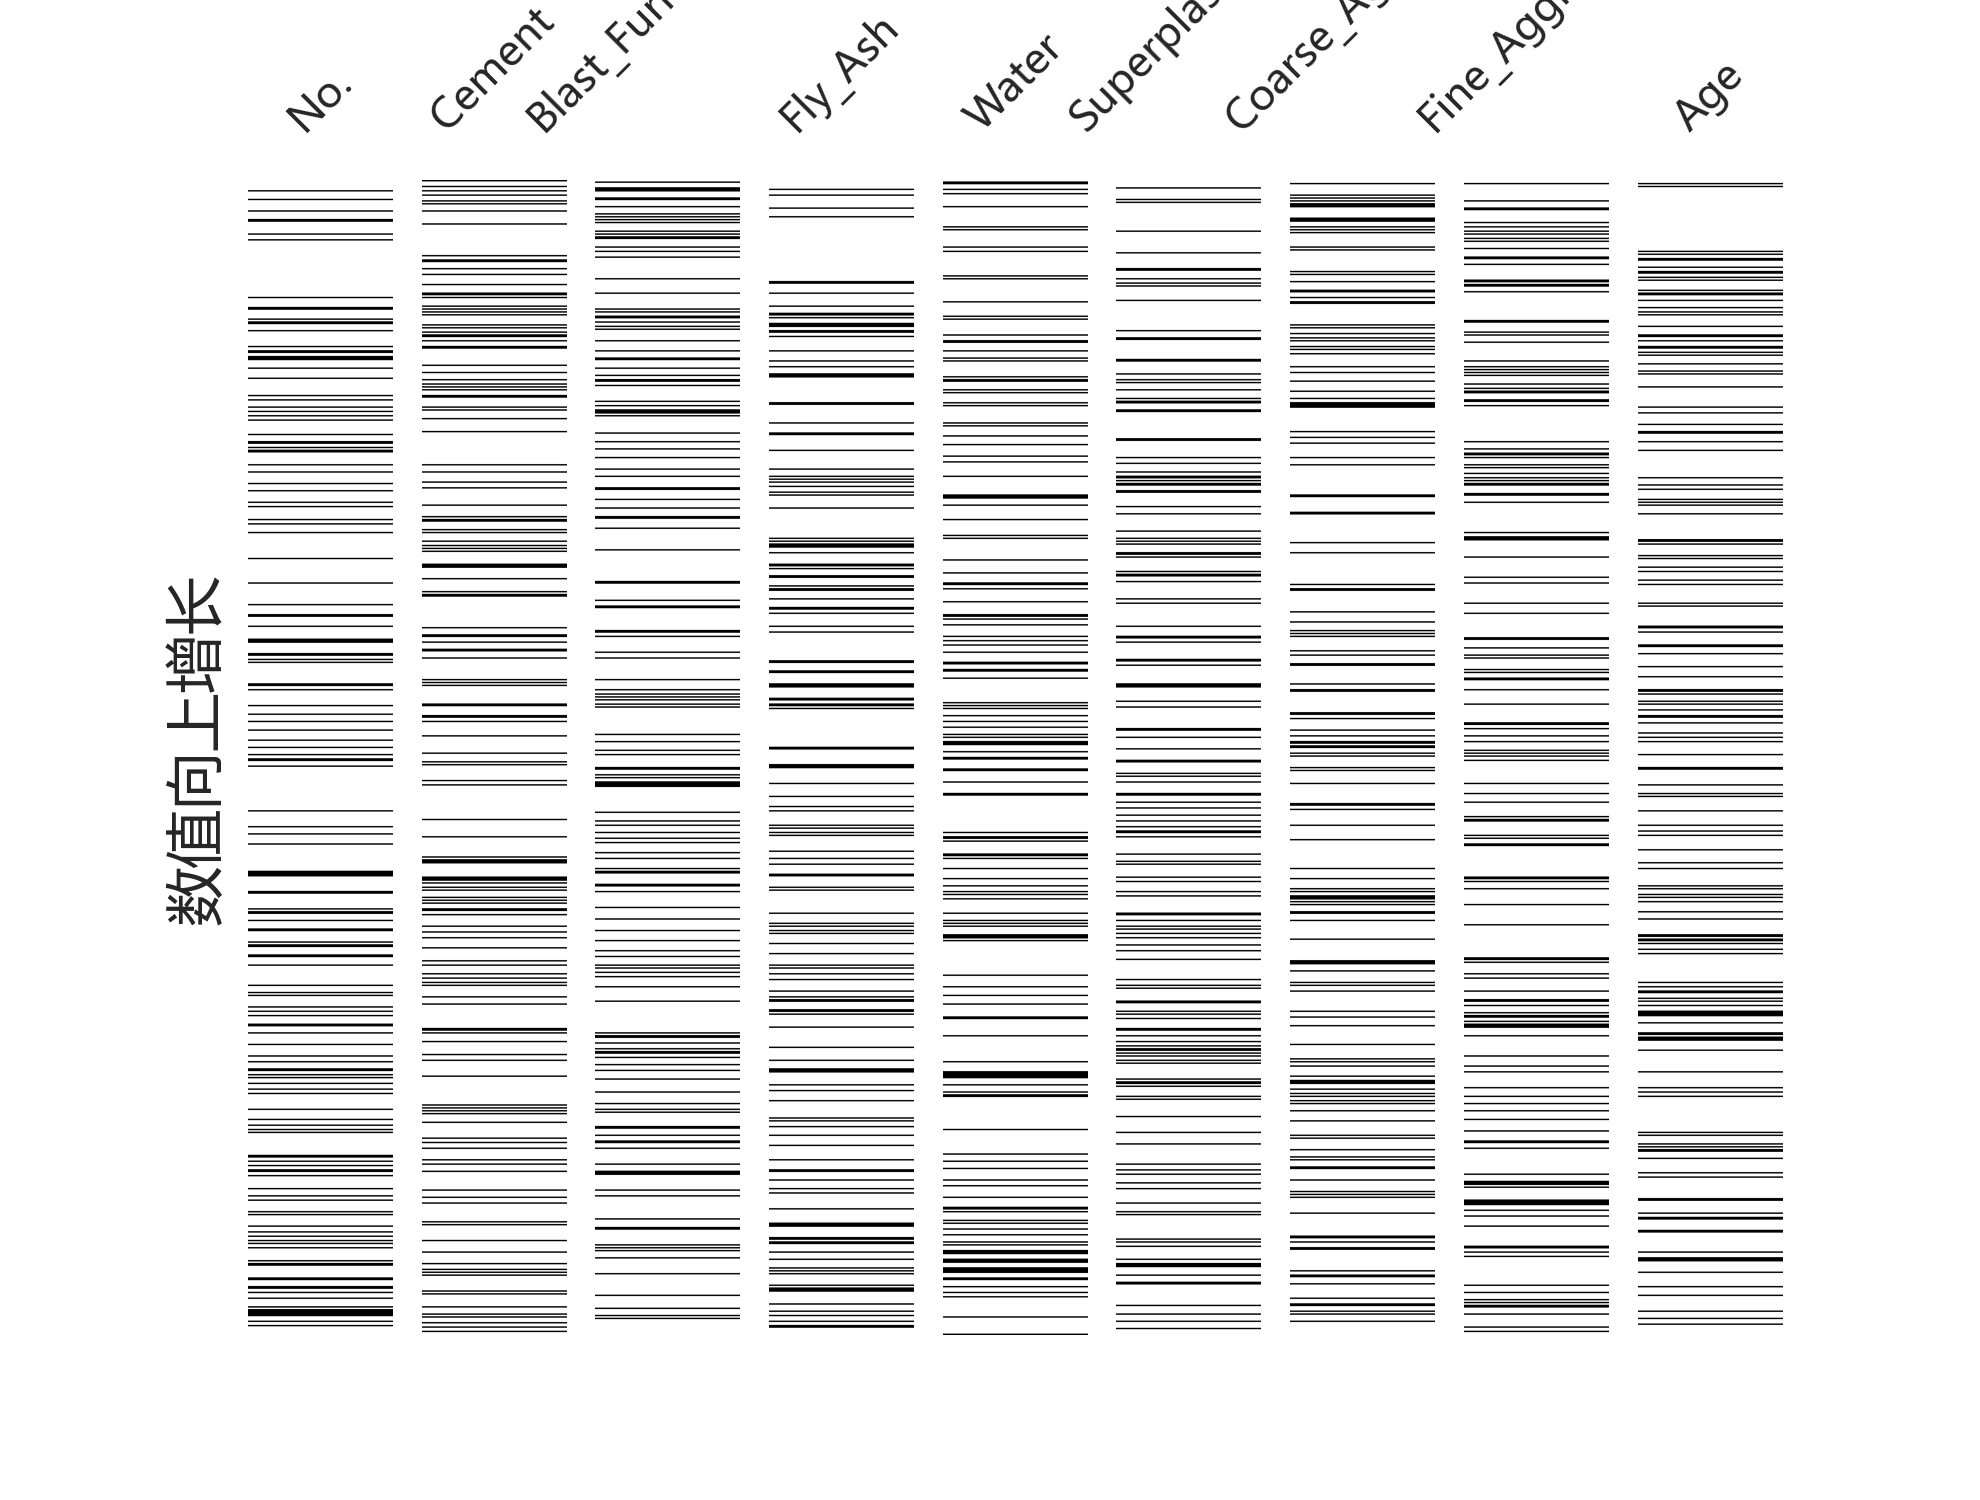
\includegraphics[scale=1]{images/missing.png}
    \caption{缺失值分布情况}\label{missing}
\end{figure}

如图\ref{correlation}所示,水泥和强塑剂配比与混凝土抗压强度呈现出正相关;养护时间也与混凝土抗压强度呈现出正相关;水的配比与混凝土抗压强度呈现出较强的负相关。

\begin{figure}[!htbp]
    \centering
    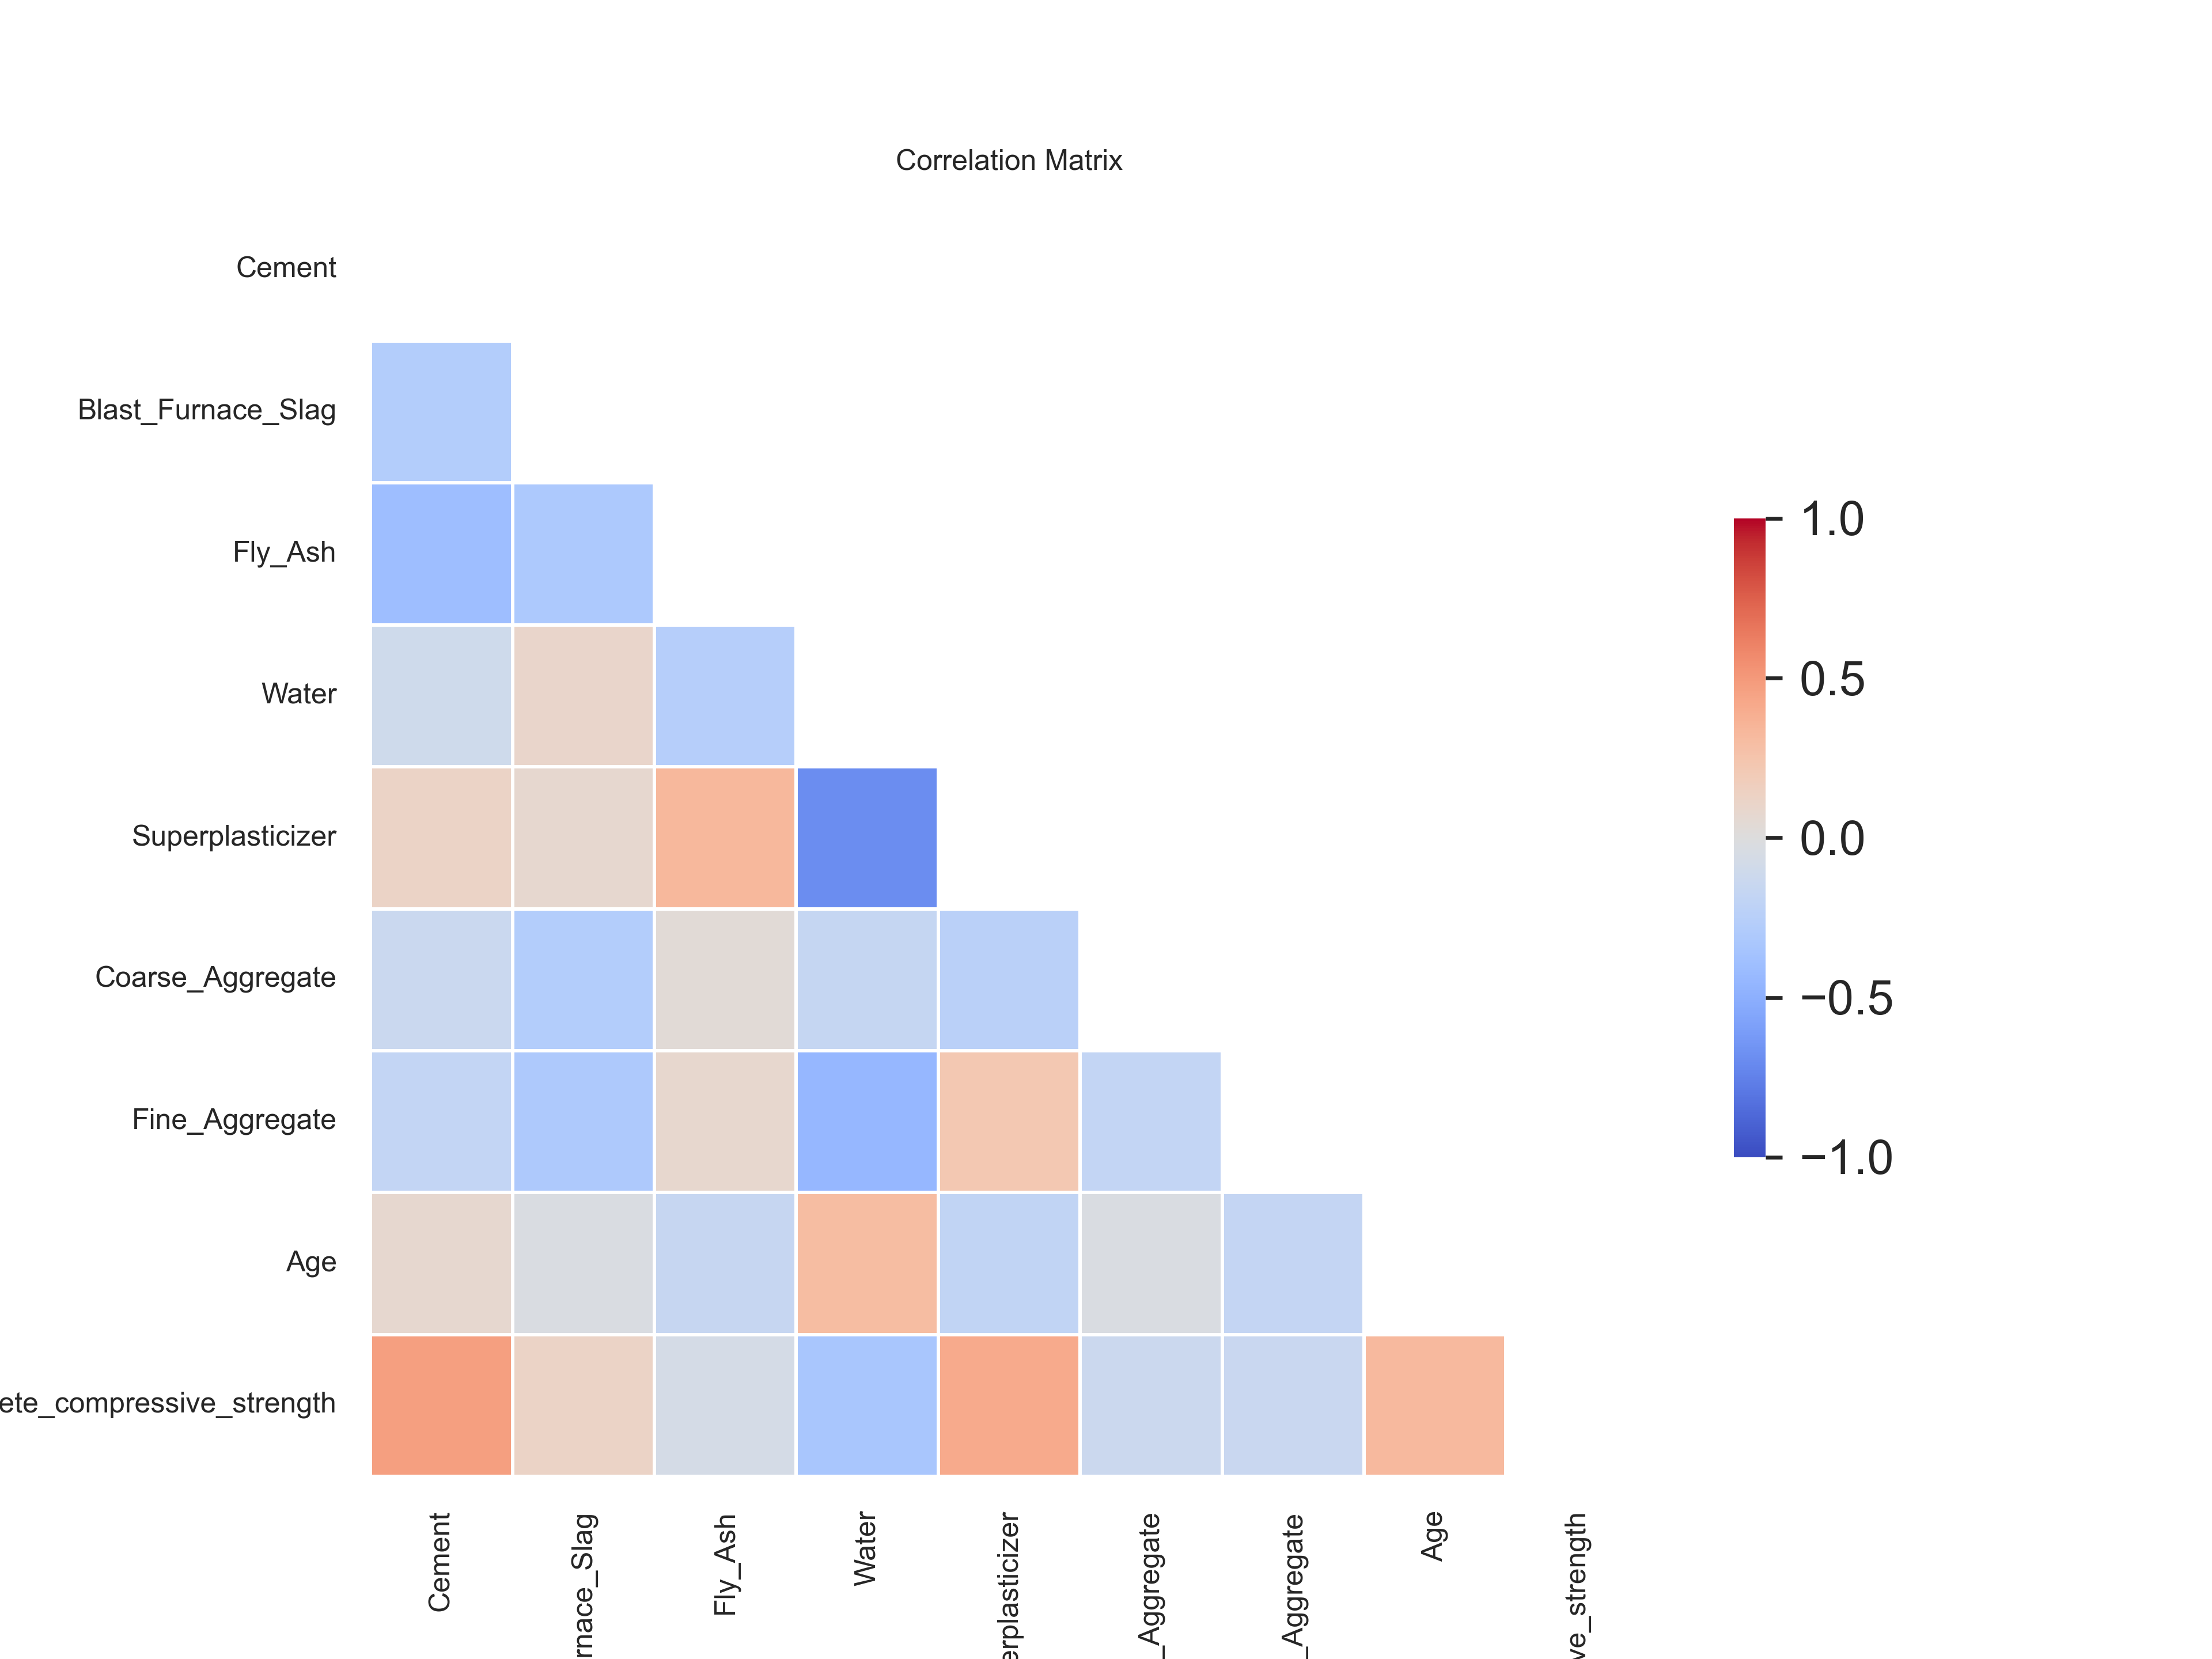
\includegraphics[scale=1]{images/correlation.png}
    \caption{相关性系数矩阵}\label{correlation}
\end{figure}

图\ref{stackplot}为各成分配比的堆叠图。

\begin{figure}[!htbp]
    \centering
    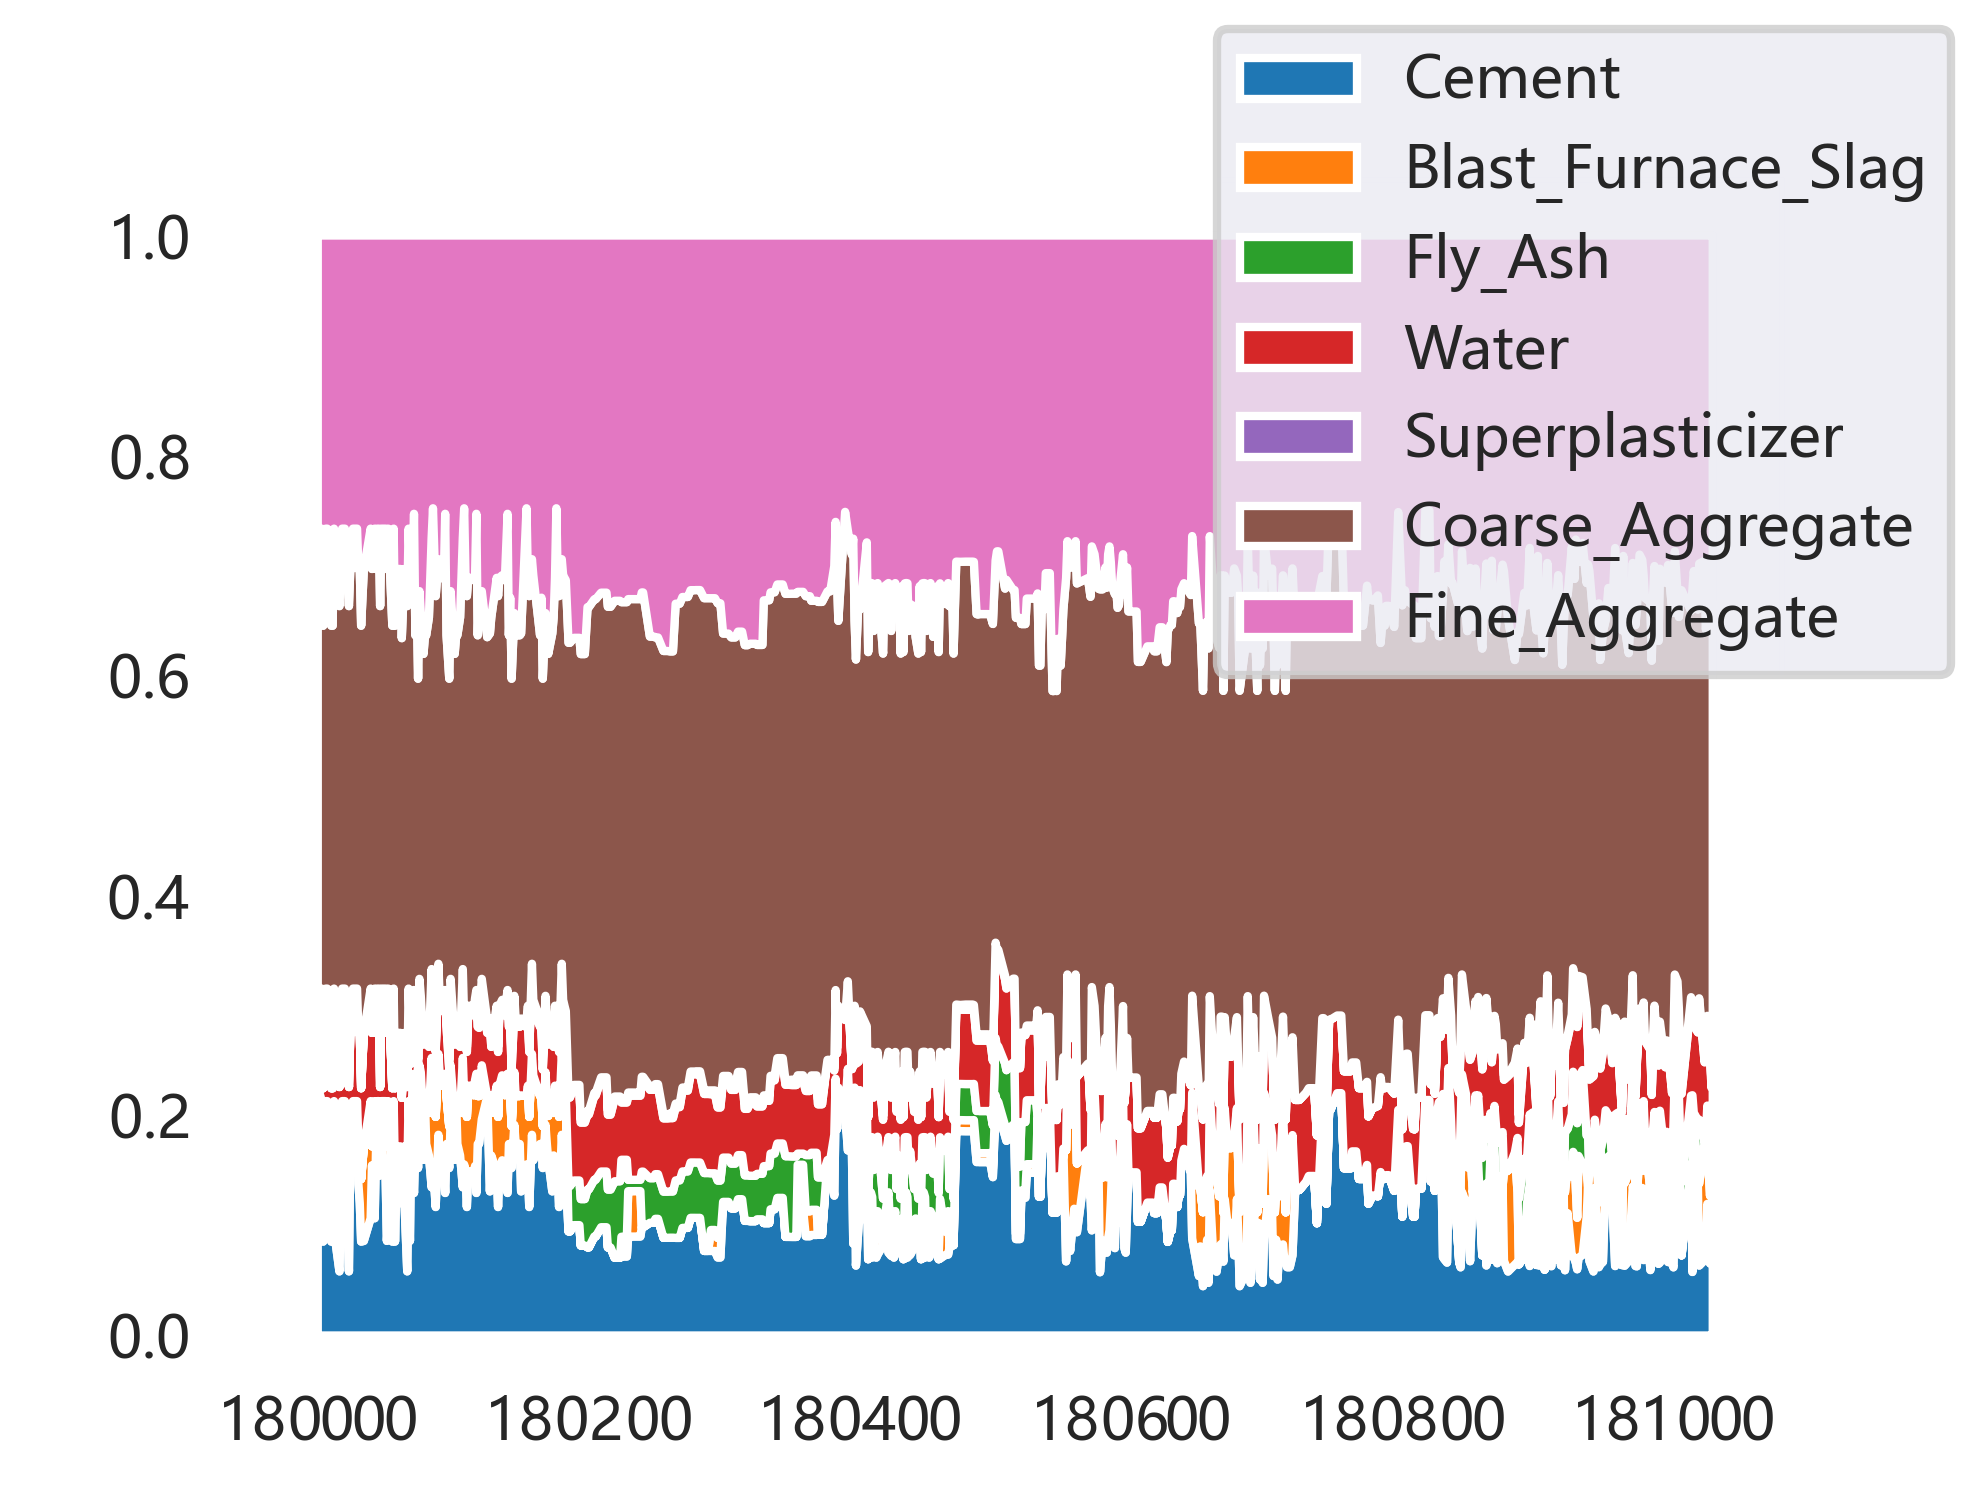
\includegraphics[scale=1]{images/stackplot.png}
    \caption{配料占比}\label{stackplot}
\end{figure}

图\ref{pairgrid}呈现出了各字段之间的关系。

\begin{figure}[!htbp]
    \centering
    \includegraphics[width=\textwidth]{images/pairgrid.png}
    \caption{下三角:各对特征的KDE图;对角线:各特征的KDE图;上三角:各对特征的RegPlot}\label{pairgrid}
\end{figure}

图\ref{hasBlast},\ref{hasFly},\ref{hasSuper}分别展示了有无高炉矿渣、飞灰和强塑剂对于混凝土抗压强度的影响。可以看出,使用高炉矿渣和强塑剂能够整体提高混凝土的抗压强度和品质的稳定性,
使用飞灰能够使得出品的混凝土抗压强度更加稳定。

\begin{figure}[!htbp]
    \centering
    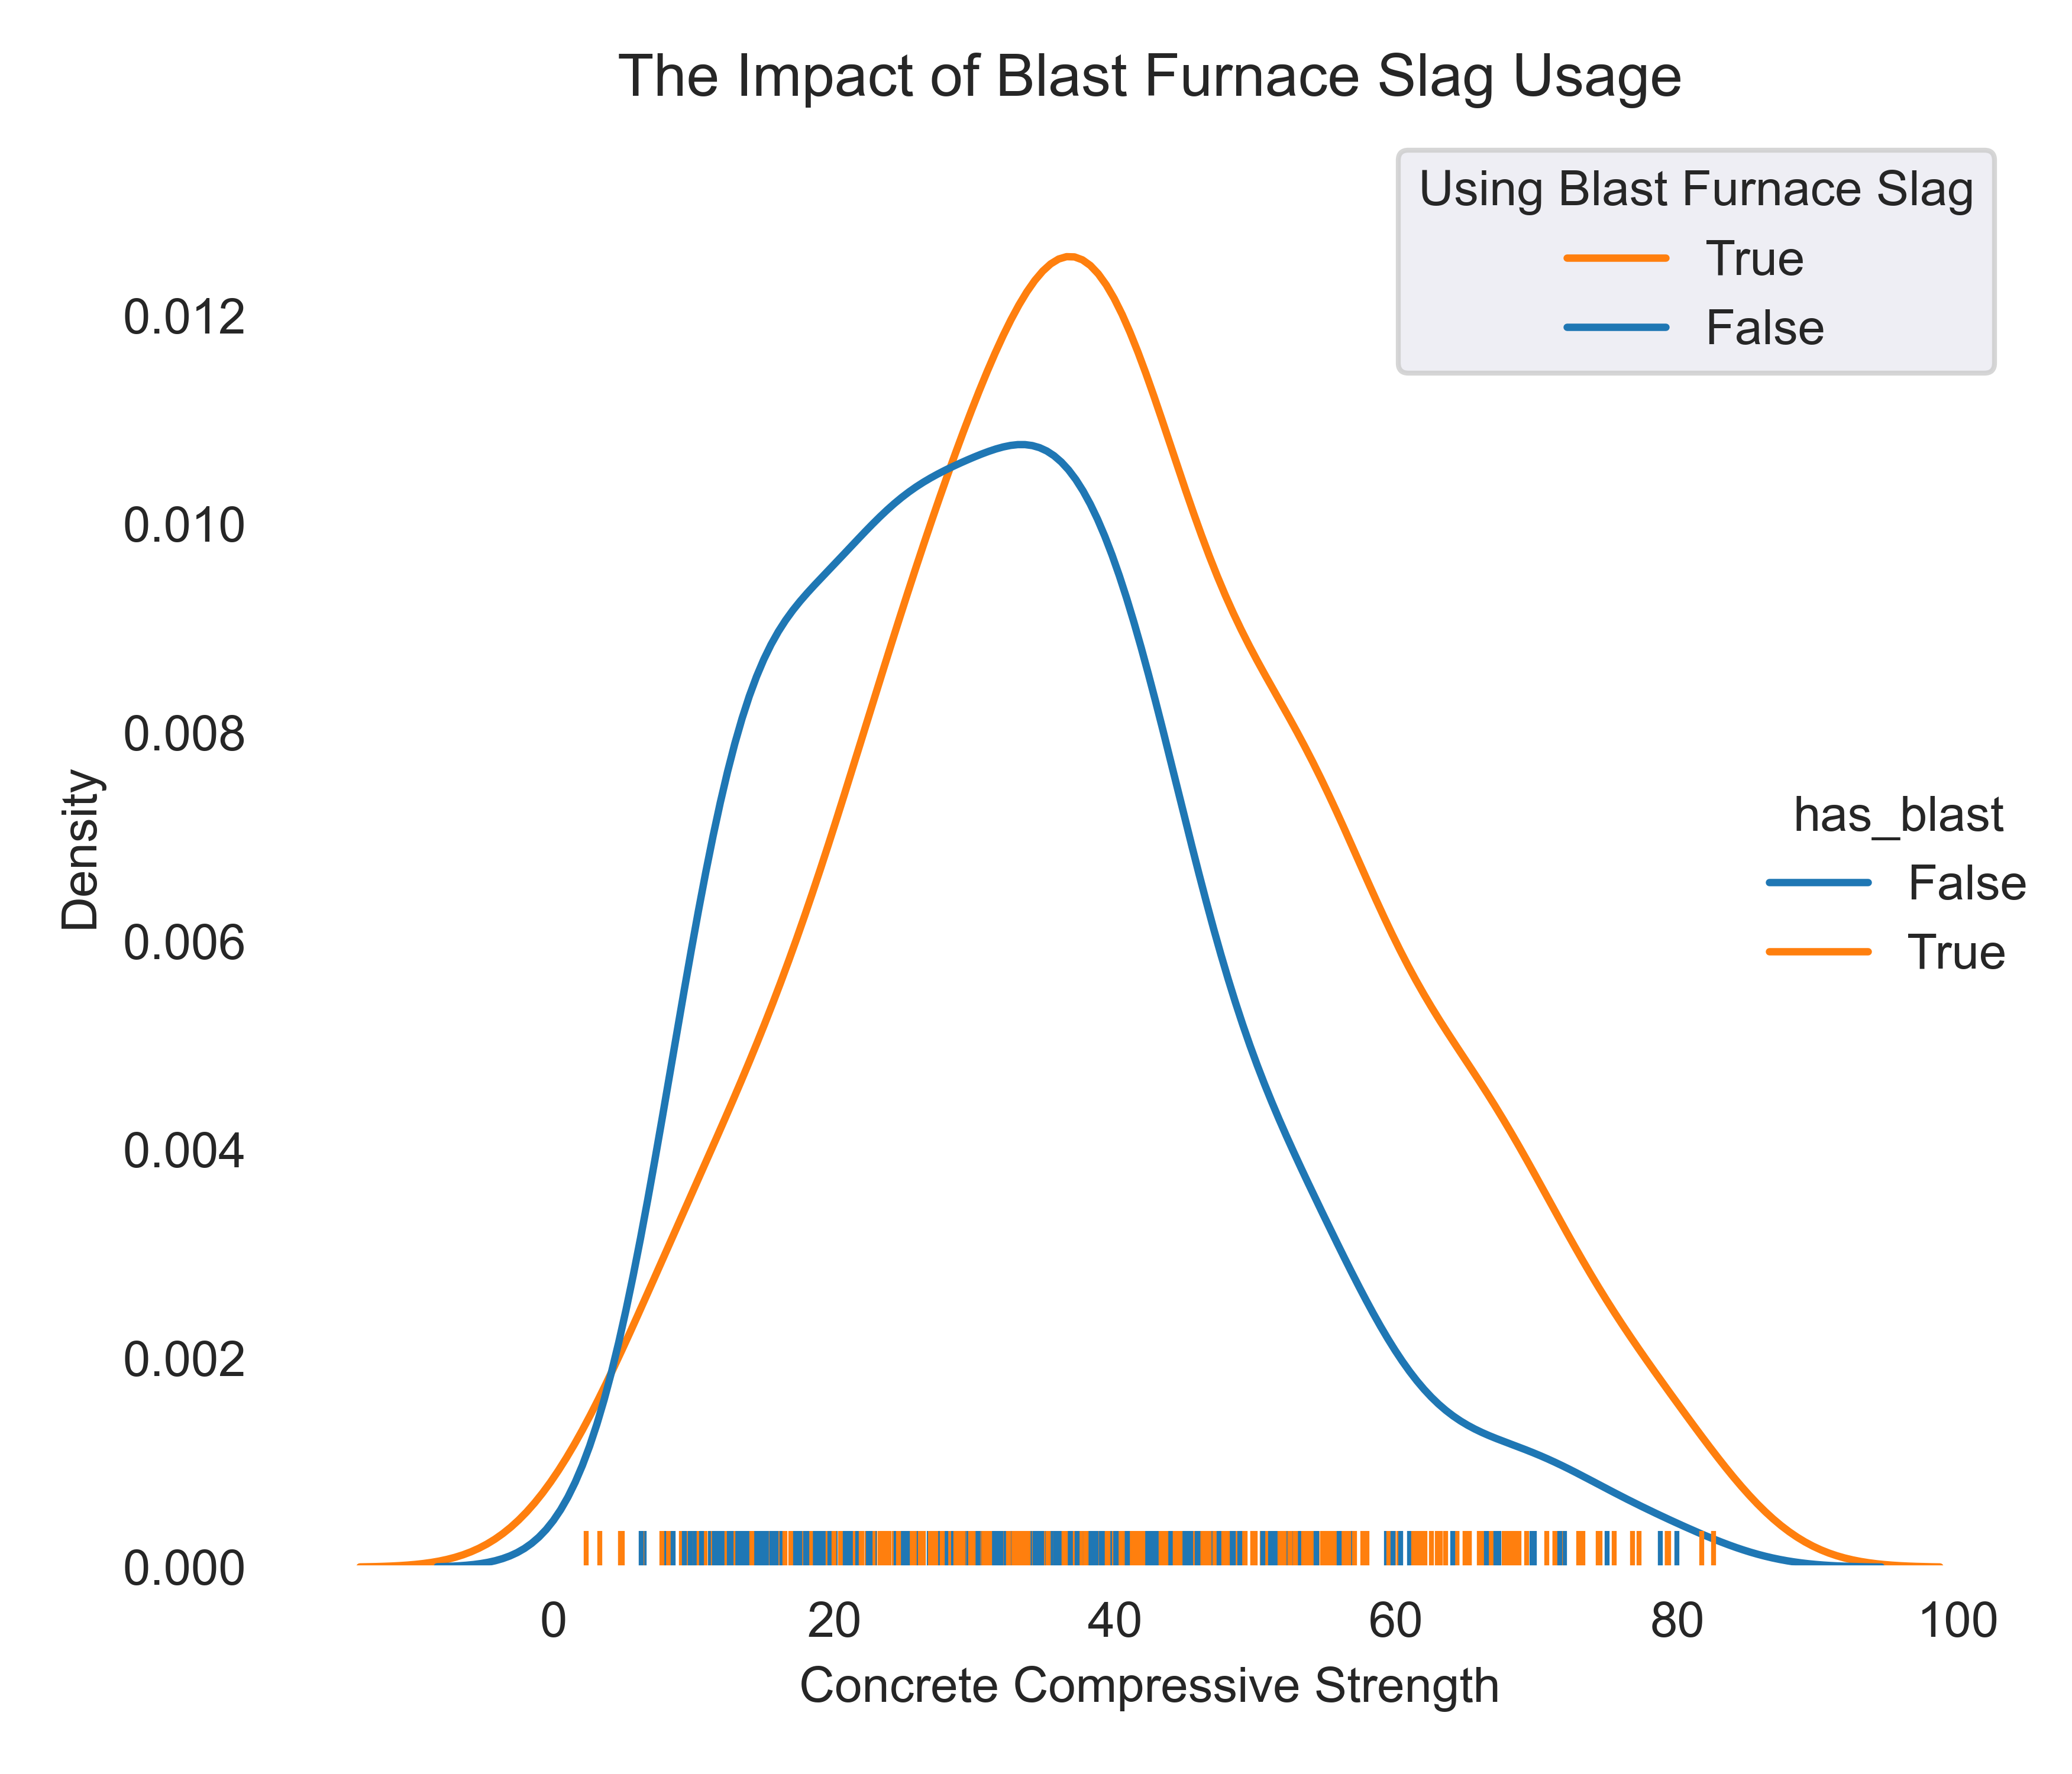
\includegraphics[scale=1]{images/has_blast.png}
    \caption{有无高炉矿渣对于混凝土抗压强度的影响}\label{hasBlast}
\end{figure}

\begin{figure}[!htbp]
    \centering
    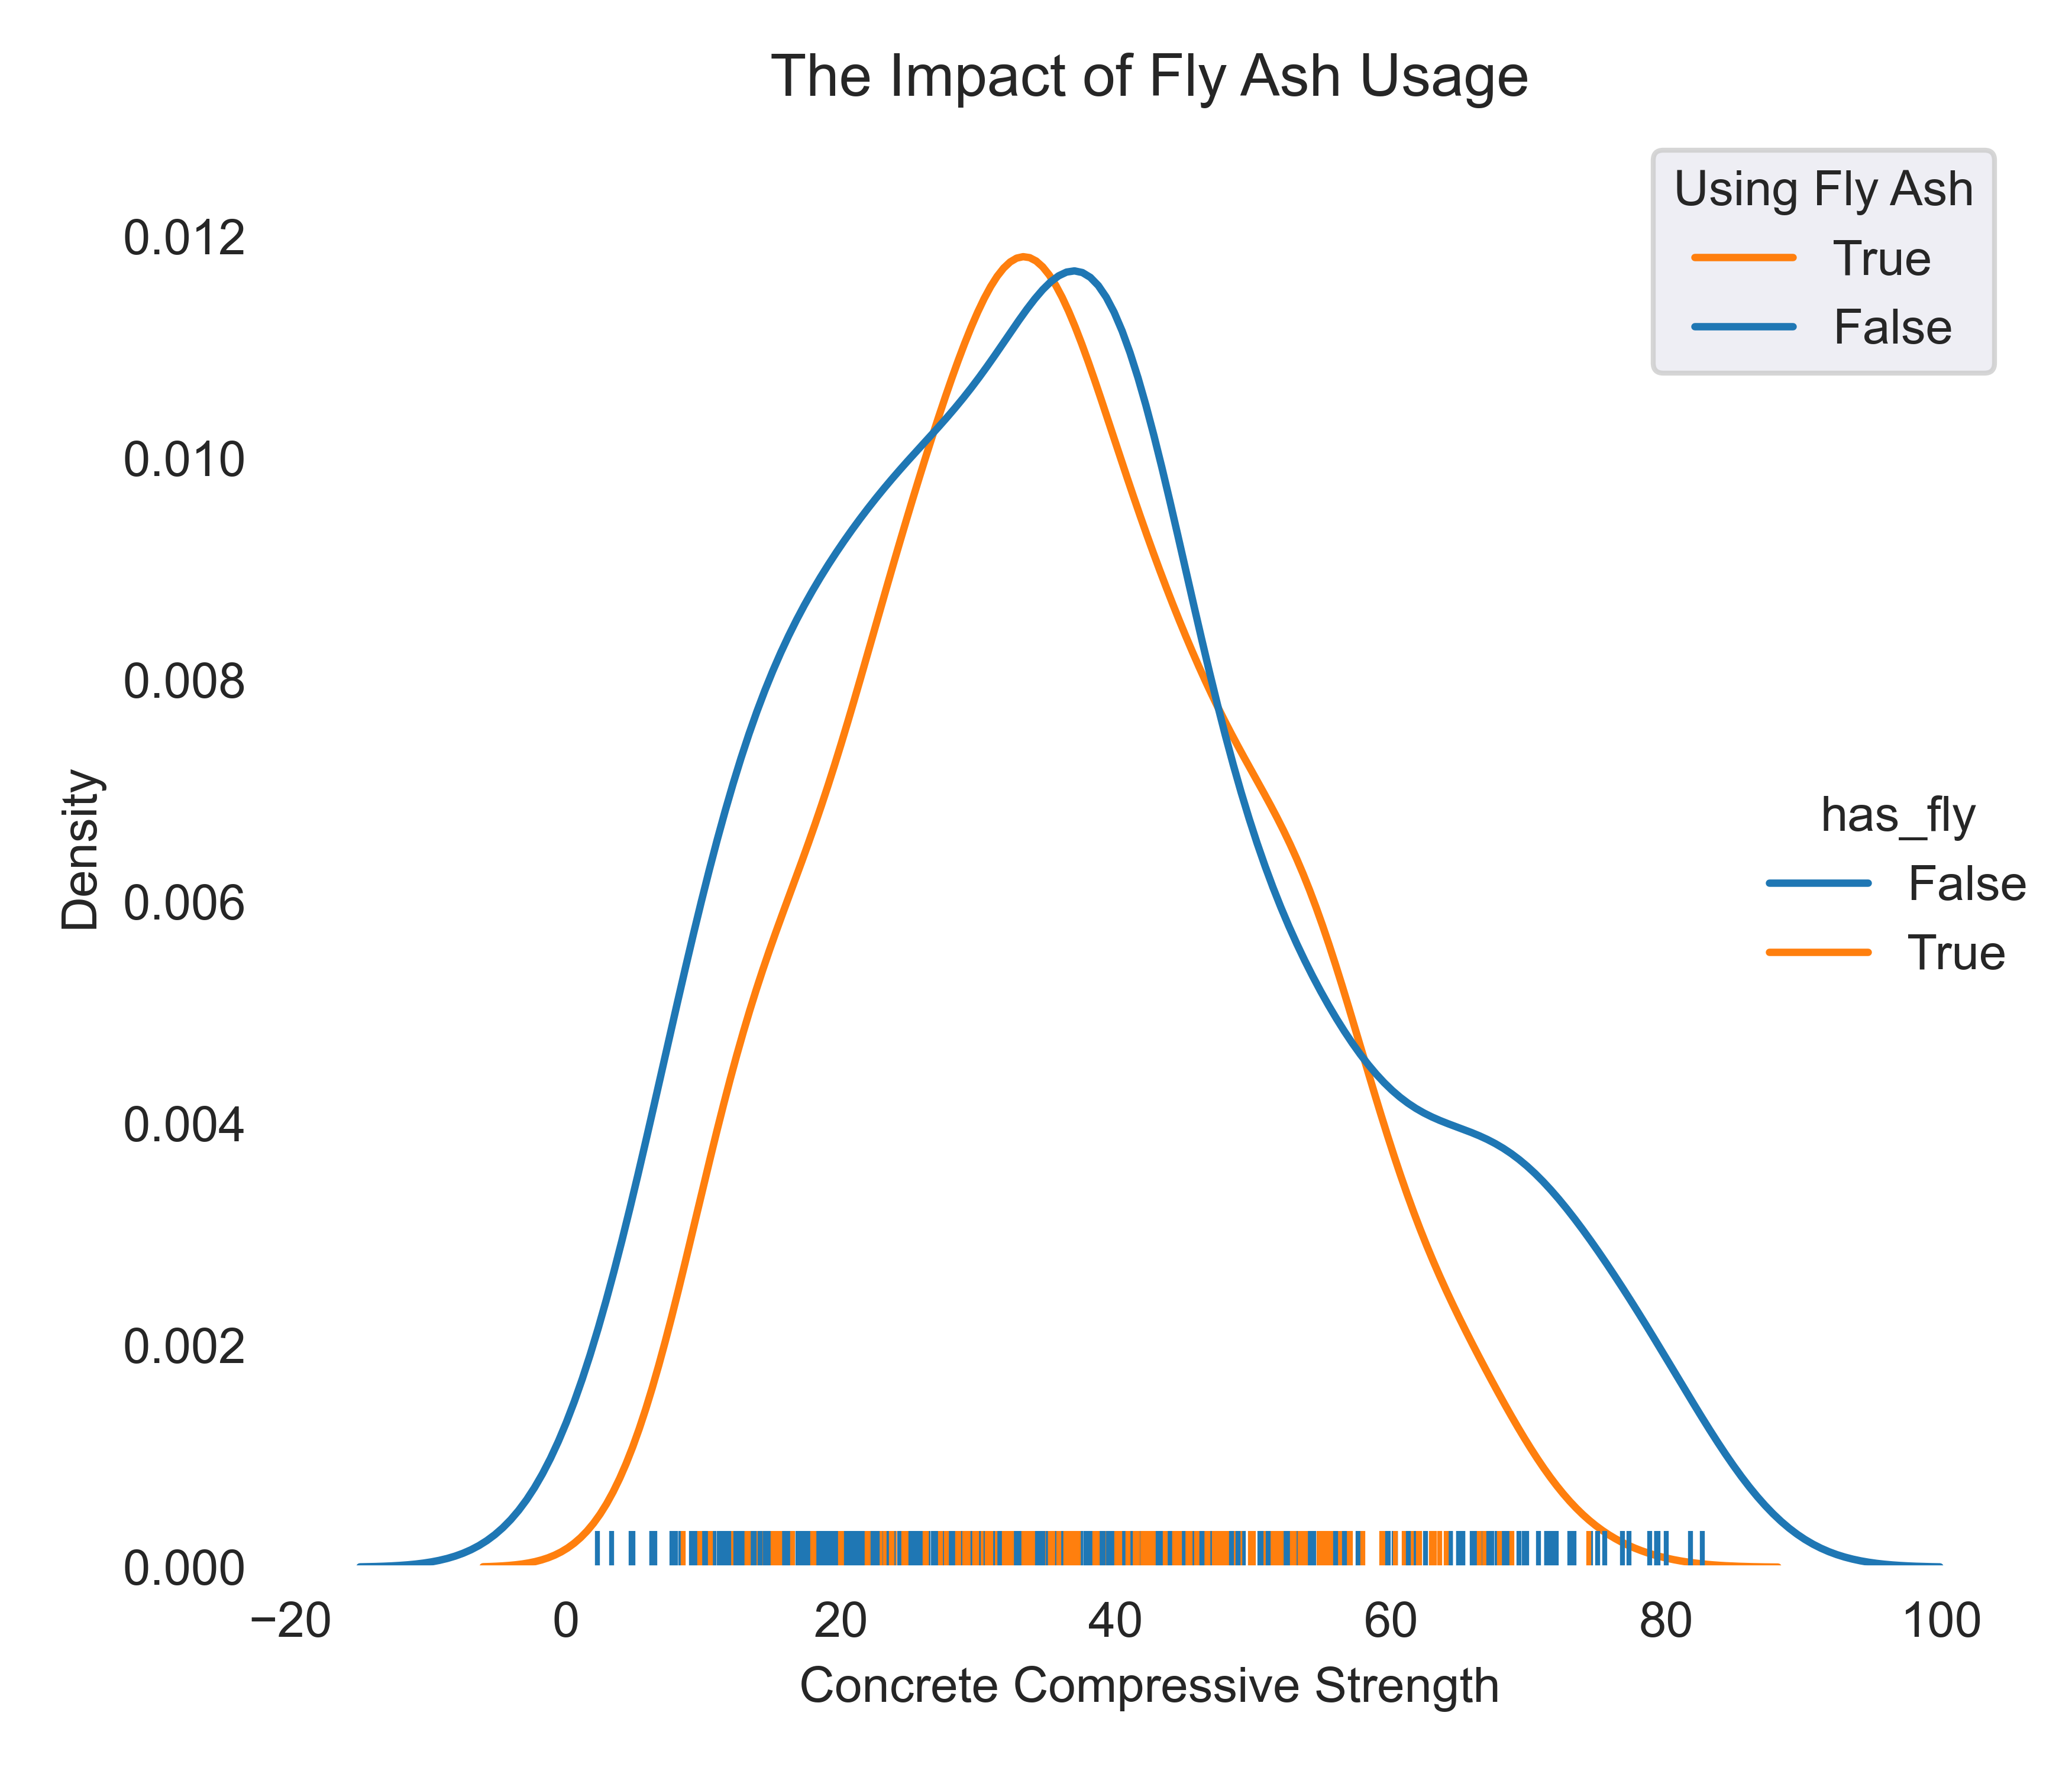
\includegraphics[scale=1]{images/has_fly.png}
    \caption{有无飞灰对于混凝土抗压强度的影响}\label{hasFly}
\end{figure}

\begin{figure}[!htbp]
    \centering
    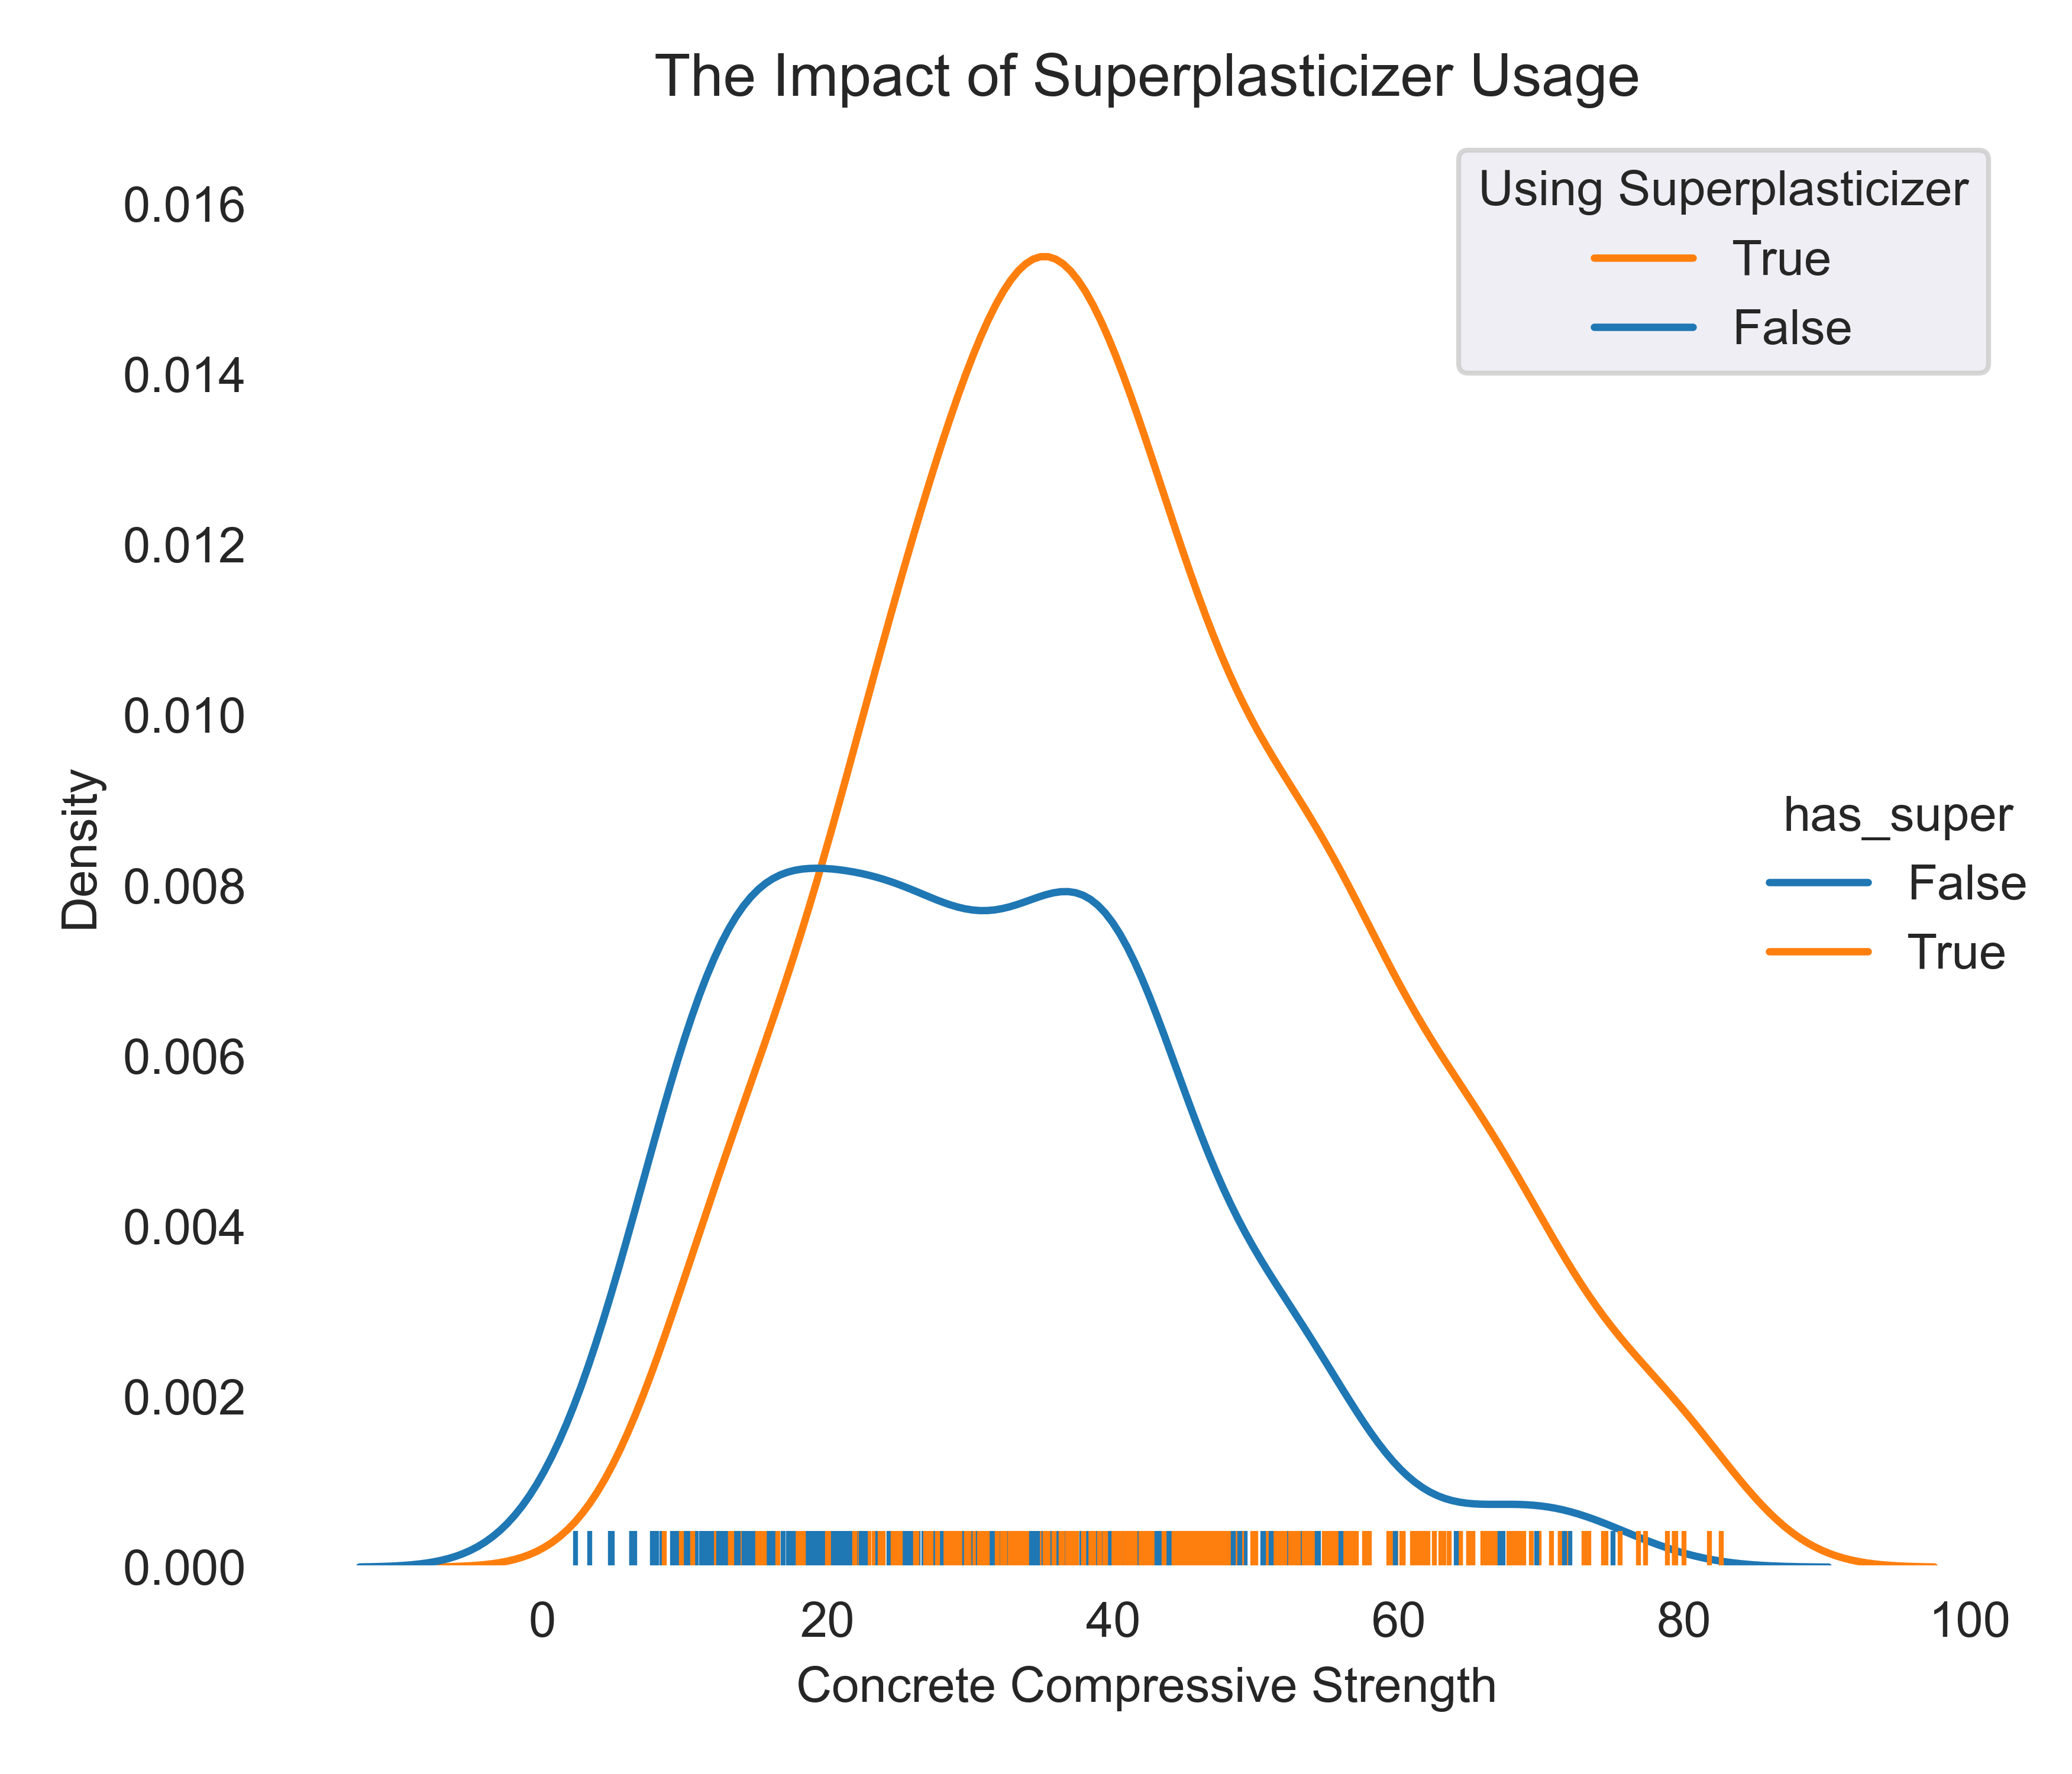
\includegraphics[scale=1]{images/has_super.png}
    \caption{有无强塑剂对于混凝土抗压强度的影响}\label{hasSuper}
\end{figure}



